\documentclass[a4paper, 11pt]{article}
\usepackage[swedish]{babel}
\usepackage{hyperref}
\usepackage[margin=0.5in]{geometry}

\usepackage{graphicx}
\usepackage{amsmath}
\usepackage[arrowdel]{physics}
\usepackage{siunitx}

\newcommand{\integ}[5][]{\int\limits_{#2}^{#3}\dd[#1]{#4}#5}

\title{Sammanfattning av EL1000 Reglerteknik, allmän kurs}
\author{Yashar Honarmandi \\ yasharh@kth.se}
\date{\today}

\begin{document}

\maketitle

\begin{abstract}
	Denna sammanfattningen innehåller centrala definitioner och satser i SF1672 Flervariabelanalys.
\end{abstract}

\pagenumbering{roman}
\thispagestyle{empty}

\newpage

\tableofcontents

\newpage

\pagenumbering{arabic}

\section{Basic Concepts in Statistical Physics}

\paragraph{Avogadro's Number}
Statistical physics discusses systems of many particles. A relevant measure of the number of particles to be studies is $N_{\text{A}} = \num{6.022e23}$.

\paragraph{Molar Mass}
The molar mass of a substance is defined as $M = mN_{\text{A}}$, where $m$ is the mass of a single atom or molecule.

\paragraph{Atomic Units}
When discussing atoms and molecules, we use relative units. These units are relative to the atomic mass unit $\au = \SI{1.66e-27}{\kilo\gram}$, defined as $\frac{1}{12}$ the mass of \ce{^{12}C}. This happens to be close to the mass of a hydrogen atom.

\paragraph{The Thermodynamic Limit}
The thermodynamic limit is the limit of the statistical consideration of a system when the number of particle is large. In this limit, quantities such as temperature, pressure and density can be defined as we know them and macroscopic equilibria can be achieved.

\paragraph{Intensive and Extensive Variables}
Intensive variables do not depend on the size of the system, whereas extensive variables do. Examples of the former are pressure and temperature, and examples of the latter are volume and total energy.

\paragraph{Heat}
Heat is the flow of energy.

\paragraph{Microstates}
A microstate of a system is any complete description of all particles in a system, for instance a specification of all positions and velocities of the particles in a gas.

\paragraph{Macrostates}
A macrostate of a system is a description of the macroscopic properties of a system.

\paragraph{Multiplicity}
The multiplicity of a macrostate is the number of microstates that yield the same macrostate.

\paragraph{The Fundamental Postulate}
The fundamental hypothesis of statistical mechanics is that all microstates available to a system have equal property.

\paragraph{Equilibrium and Multiplicity}
Combining the fundamental postulate with our knowledge of thermodynamics, it is clear that a system in thermal equilibrium has maximal multiplicity.

\paragraph{The Boltzmann constant}
Consider two systems which are not in contact. The total energy and multiplicity is given by
\begin{align*}
	E = E_{1} + E_{2},\ \Omega = \Omega_{1}(E_{1})\Omega_{2}(E_{2}).
\end{align*}
At equilibrium, the total multiplicity is maximal. Differentiating with respect to $E_{1}$ gives
\begin{align*}
	\del{E_{1}}{\Omega} = \Omega_{2}\dv{\Omega_{1}}{E_{1}} + \Omega_{1}\dv{\Omega_{2}}{E_{2}}\dv{E_{2}}{E_{1}}.
\end{align*}
The total energy is fixed, yielding
\begin{align*}
	\frac{1}{\Omega_{1}}\dv{\Omega_{1}}{E_{1}} = \frac{1}{\Omega_{2}}\dv{\Omega_{2}}{E_{2}},
\end{align*}
which we can rewrite as
\begin{align*}
	\dv{\ln{\Omega_{1}}}{E_{1}} = \dv{\ln{\Omega_{2}}}{E_{2}}.
\end{align*}
We define this to be equal to $\frac{1}{\kb T}$.

\paragraph{The Boltzmann Factor}
Consider a thermal bath in contact with a small system. The energy of the small system is $\varepsilon$, so that the bath has energy $E - \varepsilon$. Taylor expanding the multiplicity yields
\begin{align*}
	\ln{\Omega(E - \varepsilon)} \approx \ln{\Omega(E)} - \varepsilon\dv{\ln{\Omega}}{E} = \ln{\Omega(E)} - \frac{\varepsilon}{\kb T},
\end{align*}
with solution
\begin{align*}
	\Omega(E - \varepsilon) = \Omega(E)e^{-\frac{\varepsilon}{\kb T}}.
\end{align*}
This exponential factor is called the Boltzmann factor.

We note that the probability of finding the small system in the macrostate with energy $\varepsilon$ is, according to the fundamental hypothesis, proportional to $e^{-\frac{\varepsilon}{\kb T}}$.

\section{Prestanda och prestandamått}

\paragraph{Stigtid}
Stigtiden definieras som $T_{\text{r}}, = t_{2} - t_{1}$, där $y(t_{2}) = 0.9$ och $y(t_{1}) = 0.1$, med $y$ mätt i relativa enheter.

\paragraph{Insvängningstid}
Insvängningstiden definieras som $\abs{y(t) - 1} < p$ när $t > T_{\text{s}}$, med $y$ mätt i relativa enheter. $p$ är typiskt lika med $0.05$.

\paragraph{Översläng}
Överslänget definieras som $y_{\text{max}} - 1$, med $y$ mätt i relativa enheter.

\paragraph{Parametrar i svängningslika system}
Om du har ett system med ett andra ordningens polynom i överförningsfunktionens nämnare, skriv polynomet som $s^{2} + 2\zeta\omega_{0}s + \omega_{0}^{2}$. Då gäller det att
\begin{align*}
	T_{\text{r}} \propto \frac{1}{\omega_{0}},\ T_{\text{s}} \approx \frac{3}{\zeta\omega_{0}},\ M = e^{\frac{\pi\zeta}{\sqrt{1 - \zeta^{2}}}}.
\end{align*}

\paragraph{Stationärt fel}
Det stationära felet är felet som kvarstår efter lång tid.

\section{Blockschema}

\paragraph{Syftet med blockschema}
Blockschema är ett systematisk sätt att rita reglerade system på.

\paragraph{Hur funkar det?}
Betrakta blocket i figur \ref{fig:basic_block}.

\begin{figure}[!ht]
	\centering
	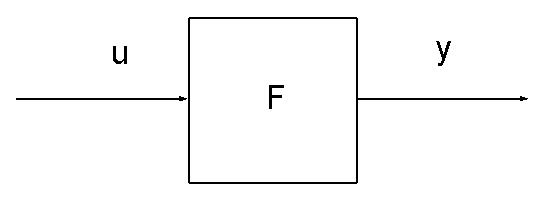
\includegraphics[width = 0.5\textwidth]{./Images/basic_block.eps}
	\caption{Illustration av ett enkelt block i ett blockschema.}
	\label{fig:basic_block}
\end{figure}

Med denna figuren menar vi exakt att $Y(s) = F(s)U(s)$.

\section{Negativ återkoppling}

\paragraph{Vad är negativ återkoppling?}
I denna kursen kommer vi att studera hur man kontrollerar ett system vid att låta avvikelsen mot det önskade värdet kontrollera regleringen av storheten.

\paragraph{Illustration i blockdiagram}
Ett enkelt negativt kontrollsystem illustrearas i figur \ref{fig:negative_feedback}.

\begin{figure}[!ht]
	\centering
	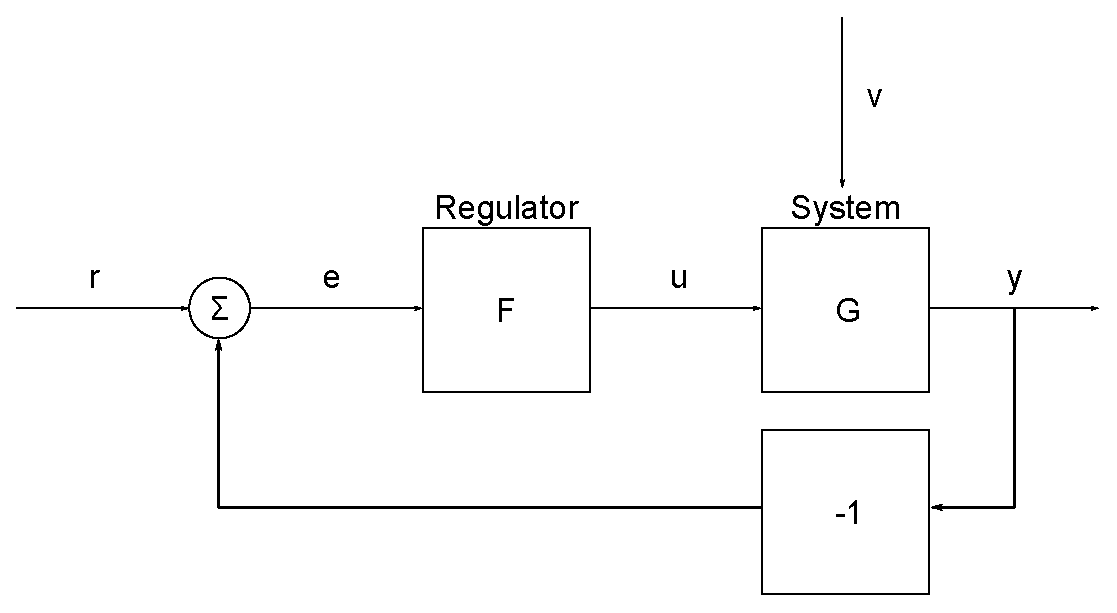
\includegraphics[width = \textwidth]{./Images/negative_feedback.eps}
	\caption{Schematisk illustration av ett enkelt negativt återkopplad system.}
	\label{fig:negative_feedback}
\end{figure}

\paragraph{Beskrivning av systemet}
Vi börjar beskrivningen av systemet med att inte betrakta störningar. I ena ändpunkten har vi
\begin{align*}
	Y = GU = GFE.
\end{align*}
Summationskomponenten till vänster ger oss
\begin{align*}
	E = R - Y,
\end{align*}
och därmed
\begin{align*}
	Y = GFR - GFY.
\end{align*}
Därmed kan vi skriva
\begin{align*}
	Y = \frac{GF}{1 + GF}R.
\end{align*}

\paragraph{Återkopplad överföringsfunktion}
För ett återkopplad system som kan skrivas som $Y = G_{\text{C}}R$ definieras $G_{\text{C}}$ som den återkopplade överföringsfunktionen. För systemet ovan har vi alltså
\begin{align*}
	G_{\text{C}} = \frac{GF}{1 + GF}R.
\end{align*}

\paragraph{Samband mellan reglerfel och referens}
Alternativt kan vi lösa systemet ovan för att få
\begin{align*}
	R - E = GFE,\ E = \frac{1}{1 + GF}R.
\end{align*}

\paragraph{Samband mellan referens och insignal}
Systemet ovan kan även lösas för att ge
\begin{align*}
	U = FR - FY = FR - GFU,\ U = \frac{F}{1  + GF}R.
\end{align*}

\paragraph{Slutna systems poler}
Vi ser att slutna system har poler där $1 + GF = 0$. Därmed bestäms systemets stabilitet av systemet och regulatorn.

\paragraph{P-reglering}
Principet i P-reglering är att välja en styrsignal som är proportionell mot storleken av felet, alltså
\begin{align*}
	u = K(r - y) = Ke.
\end{align*}
Det är här klart att för att få negativ återkoppling väljer vi $K > 0$.

Denna regleringsmetoden
\begin{itemize}
	\item minskar inverkan av störning och modellfel för ett bra val av $K$.
	\item ökar snabbheten vid insvängning.
	\item stabiliserar instabila system.
\end{itemize}
Däremot kan regleringen gå fel om t.ex.
\begin{itemize}
	\item systemet inte uppför sig som man tror.
	\item man har begränsningar i styrförmåga.
	\item man får instabilitet på grund av återkopplingen.
\end{itemize}

Det är även ett problem att om felet är stationärt, är även styrsignalen det, så även om du har ett nollskild fel klarar inte systemet nödvändigtvis anpassa sig.

\paragraph{PID-reglering}
PID står för proportionell integrerande deriverande. Denna sortens reglering löser många reglerproblem. Med PID-reglering väljer vi styrsignlaen
\begin{align*}
	u = K_{\text{P}}e + K_{\text{I}}\integ{t_{0}}{t}{\tau}{e} + K_{\text{D}}\dv{e}{t}.
\end{align*}
Alternativt kan vi skriva det som
\begin{align*}
	u = K\left(e + \frac{1}{T_{\text{I}}}\integ{t_{0}}{t}{\tau}{e} + T_{\text{D}}\dv{e}{t}\right).
\end{align*}

De tre ingående termerna i styrsignalen är
\begin{itemize}
	\item proportionell återkoppling, som betraktar det nuvarande felet.
	\item integrerande återkoppling, som betraktar hur felet har uppfört sig.
	\item deriverande återkoppling, som betraktar hur felet kommer att uppföra sig.
\end{itemize}

\paragraph{PI-reglering}
PI-reglering använder ej den deriverande återkopplingstermen. Vi ser härifrån att vid ett stationärt tillstånd är antingen $e = 0$, annars ökar eller minskar $u$ på grund av integraltermen.

Vi vill nu betrakta systemets insvängning. Om det stationära $\bar{u}$ krävs för att $e = 0$, har vi
\begin{align*}
	\bar{u} = K\left(e + \frac{1}{T_{\text{I}}}\integ{t_{0}}{t}{\tau}{e}\right).
\end{align*}
Vid att derivera detta fås
\begin{align*}
	K\left(\dv{e}{t} + \frac{1}{T_{\text{I}}}e\right) = 0,
\end{align*}
med lösning proportionell mot $e^{-\frac{t}{T_{\text{I}}}}$.

Notera att om man har stort fel kan PI-reglering ge problem. Därför använder man det typiskt när felen är små.

\paragraph{PI-reglering i Laplacevärlden}
Vid att Laplacetransformera uttrycket för styrsignalen i en PI-regulator, nämligen
\begin{align*}
	u = K\left(e + \frac{1}{T_{\text{I}}}\integ{t_{0}}{t}{\tau}{e}\right),
\end{align*}
fås
\begin{align*}
	U = K\left(E + \frac{1}{T_{\text{I}}s}E\right),
\end{align*}
och enligt figur \ref{fig:negative_feedback} ser vi att
\begin{align*}
	F(s) = K\left(1 + \frac{1}{T_{\text{I}}s}\right).
\end{align*}

\section{Frekvensanalys}

\paragraph{Fundamental ide}
Eftersom periodiska funktioner kan skrivas som en summa av trigonometriska funktioner och funktioner som avtar tillräcklig snabbt kan skrivas som en integral över trigonometriska funktioner, vet vi att när vi studerar linjära system räcker det att studera systemets respons på en enda term, alltså en enda trigonometrisk funktion, och se hur den beror av frekvensen. Om vi tillför en signal $u = \sin{\omega t}$ till ett system med överförningsfunktion $G$ får vi
\begin{align*}
	y &= \integ{0}{\infty}{\tau}{g(\tau)u(t - \tau)} \\
	  &= \Im\left(\integ{0}{\infty}{\tau}{g(\tau)e^{i\omega(t - \tau)}}\right) \\
	  &= \Im\left(e^{i\omega t}\integ{0}{\infty}{\tau}{g(\tau)e^{-i\omega\tau}}\right) \\
	  &= \Im(e^{i\omega t}G(i\omega)) \\
	  &= \abs{G(i\omega)}\sin(\omega t + \arg{G(i\omega)}).
\end{align*}
Det kan även finnas transienta termer här, men om systemet är stabilt kommer dessa försvinna över tid. Vi ser alltså att systemets svar beror av $G(i\omega)$.

\paragraph{Nyquistdiagram}
Ett Nyquistdiagram är en uppritning av $G(i\omega)$ för $0 < \omega < \infty$.

\paragraph{Bodediagram}
Ett Bodediagram är en uppritning av $\abs{G(i\omega)}$ och $\arg{G(i\omega)}$ som funktioner av $\omega$.

\paragraph{Bandbredd}
Bandbredden är bredden på det frekvensintervallet där $\abs{G(i\omega} \geq \frac{1}{\sqrt{2}}$, och benämnas $\omega_{\text{B}}$. Bandbredden kan ge information om systemets tillväxt, då hög bandbredd typiskt betyder snabb tillväxt. Man önskar typiskt att denna skall vara stor.

\paragraph{Resonansfrekvens}
Resonansfrekvensen $\omega_{\text{r}}$ är den frekvens som ger starkast respons i systemet.

\paragraph{Resonanstopp}
Resonanstoppen är $M_{\text{p}} = \abs{G(i\omega_{\text{r}})}$, och ger typiskt en indikation på hur mycket översläng man får. Man önskar typiskt att denna ska vara liten.

\paragraph{Stationärt fel}
Det stationära felet ges av $e_{0} = 1 - G_{\text{C}}(0)$.

\paragraph{Brytningspunkter}
Om överförningsfunktionen kan skrivas som
\begin{align*}
	G(i\omega) = \frac{\prod(i\omega - z_{i})}{\prod(i\omega - p_{i})},
\end{align*}
är alla $z_{i}$ och $p_{i}$ brytningspunkter för systemet. Här kommer de största lutningsändringarna i Bodediagrammet.

\paragraph{Bodes relation}
Låt $G$ vara minimumsfas, dvs. ha alla sina nollställen och poler i vänstre halvplan, och $G(0) > 0$. Då gäller att om $\abs{G(i\omega)}$ i ett visst frekvensområde avtar med \SI{20}{\deci\bel} per dekad (en dekad är en ökning i frekvens med en faktor $10$), är $\arg{G(i\omega)}\approx \SI{-90}{\degree}$, och om $\abs{G(i\omega)}$ avtar med \SI{40}{\deci\bel} per dekad, är $\arg{G(i\omega)}\approx \SI{-180}{\degree}$.

\paragraph{Snabbhet och svängighet}
Vi kan med tidigare resultat se att om $G_{\text{O}}(i\omega)$ är nära $1$ blir $G_{\text{C}}(i\omega)$ stor, och om $G_{\text{O}}(i\omega)$ är liten blir även $G_{\text{C}}(i\omega)$ liten. Vi kan också se att ett ekvivalent kriterium för bandbredden är $\abs{G_{\text{O}}(i\omega) - 1} \leq \sqrt{2}$ för $\omega \geq \omega_{\text{B}}$.

\paragraph{Resonanstopp och fasmarginal}
Vi har
\begin{align*}
	M_{\text{p}} \geq \abs{G(i\omega_{\text{c}})} = \frac{1}{2\sin(\frac{1}{2}\phi_{\text{m}})}.
\end{align*}
Speciellt ger liten fasmarginal stort översläng.

\section{Kompensering}

\paragraph{Ideen}
Vi ser att det enklaste sättet att konstruera en bra regulator på är att ändra konstruktionen av det öppna systemet. Vi bestämmer alltså regulatorn $F$ utifrån krav på
\begin{itemize}
	\item snabbhet, alltså skärfrekvens.
	\item dämpning, alltså fasmarginal.
	\item stationärt fel, alltså krav på $\abs{G_{\text{O}}(0)}$.
\end{itemize}

\paragraph{Kompensation för snabbhet}
För snabbhet räcker det med en P-regulator. Denna flyttar amplitudkurvan, men ändrar ej faskurvan. Alltså hjälper den oss att bestämma skärfrekvensen.

\paragraph{Fasavancering}
För att höja fasen kan man använda en deriverande länk, alltså en regulator med överföringsfunktion
\begin{align*}
	F = K(\tau_{\text{D}}s + 1).
\end{align*}
Typiskt kan man inte låta deriveringen verka fullt ut, så överförningsfunktionen blir i stället på formen
\begin{align*}
	F_{\text{lead}} = K\frac{\tau_{\text{D}}s + 1}{\beta\tau_{\text{D}}s + 1}.
\end{align*}
Vi har
\begin{align*}
	\arg{F_{\text{lead}}} = \dots = \arctan{\frac{(1 - \beta)\tau_{\text{D}}\omega}{1 + \beta\tau_{\text{D}}^{2}\omega^{2}}},
\end{align*}
och får därmed att den maximala fasförskjutningen är
\begin{align*}
	\phi_{\text{max}} = \arctan{\frac{1 - \beta}{2\sqrt{\beta}}}
\end{align*}
för frekvensen
\begin{align*}
	\omega = \frac{1}{\sqrt{\beta}\tau_{\text{D}}}.
\end{align*}

\paragraph{Lågfrekvensförstärkning}
Lågfrekvensförstärkning kan ta bort stationärt fel. För att lågfrekvensförstarka kan man använda en integrerande länk, alltså en regulator med överförningsfunktion
\begin{align*}
	F = \frac{\tau_{1}s + 1}{\tau_{\text{D}}s}.
\end{align*}
Denna har dock oändligt hög förstärkning för låga frekvenser, kan man i stället använda en fasretarderande länk, alltså en regulator med överförningsfunktion
\begin{align*}
	F_{\text{lag}} = \frac{\tau_{1}s + 1}{\beta\tau_{1}s + \gamma}.
\end{align*}
Vi har
\begin{align*}
	\arg{F_{\text{lag}}} = \dots = -\arctan{\frac{(1 - \gamma)\tau_{1}\omega_{\text{c}}}{\gamma + \tau_{1}^{2}\omega_{\text{c}}^{2}}}.
\end{align*}
Det kan däremot vara svårt att göra rätt val av parametrar.

\paragraph{Arbetsgång}
Arbetsgången i kompensering är att
\begin{itemize}
	\item bestämma önskad bandbredd.
	\item bestämma önskad fasmarginal för att ge nödvändig fasökning vid skärfrekvensen.
	\item Gör lead- och laggrejer. Jag kanske borde fatta det.
\end{itemize}

\end{document}
